\documentclass[a4paper, 12pt, openany]{book}

\usepackage[utf8]{inputenc}
\usepackage[T1]{fontenc}
\usepackage[brazil]{babel}
\usepackage{indentfirst}
\usepackage{verbatim}
\usepackage{listings}
\usepackage{color}
\usepackage[top=2cm, bottom=2cm, left=2cm, right=3cm]{geometry}
\usepackage{tikz}
\usetikzlibrary{circuits}
\usepackage{amsmath}
\usepackage{graphicx}

\newtheorem{example}[subsubsection]{Exemplo}

%Para trechos maiores de código, utilizar o lstlisting. Para trechos menores, utilizar o verbatim

\definecolor{dkgreen}{rgb}{0,0.6,0}
\definecolor{gray}{rgb}{0.5,0.5,0.5}
\definecolor{mauve}{rgb}{0.58,0,0.82}

\lstset{
  language=Scilab,                
  basicstyle=\footnotesize,           
  numbers=left,                   
  numberstyle=\tiny\color{gray},  
  stepnumber=2,                             
  numbersep=5pt,                  
  backgroundcolor=\color{gray!10},    
  showspaces=false,               
  showstringspaces=false,         
  showtabs=false,                 
  frame=single,                   
  rulecolor=\color{black},        
  tabsize=2,                      
  captionpos=b,                   
  breaklines=true,                
  breakatwhitespace=false,        
  title=\lstname,                               
  keywordstyle=\color{blue},          
  commentstyle=\color{dkgreen},       
  stringstyle=\color{mauve},     
}

\title{\Huge Controle de Sistemas Lineares com Scilab}
\author{Org: Victor Santos Nunes}
\date{2020}

\begin{document}
    \frontmatter
    
    \maketitle
    
    %\listoffigures
    %\listoftables
    \tableofcontents
    
    \chapter{Agradecimentos}
    \input{CapitulosIniciais/agradecimentos}
    
    \chapter{Prefácio}
    Este material não tem a pretensão de esgotar o assunto tratado aqui. A ideia é mostrar formas práticas de resolver certos problemas que surgem no estudo da teoria de controle.
    
    \mainmatter
    
    \part{Pré-Requisitos}
    
    \chapter{Espaço de Estados e Função de Transferência}
    \section{Representando Função de Transferência no Scilab}

%Para trechos maiores de código, utilizar o lstlisting. Para trechos menores, utilizar o verbatim
% \begin{lstlisting}
%     s=%s;
%     G = (6.3223*s^2+18*s+12.8112)/(s^4+6*s^3+11.3223*s^2+18*s+12.8112);
% \end{lstlisting}

%Depois utilizar Tikz para fazer diagrama de bloco aqui

Quero representar a função de transferência abaixo no Scilab:
\\
\\
$$G(s) = \frac{6.3223s^{2}+18s+12.8112}{s^{4}+6s^{3}+11.3223s^{2}+ 18s + 12.8112  
}$$

Para fazer isso eu posso escrever as seguintes linhas de código:

\begin{verbatim}
    --> s = %s;
    --> G = (6.3223*s^2+18*s+12.8112)/(s^4+6*s^3+11.3223*s^2+18*s+12.8112);
\end{verbatim}

Na primeira linha, onde vemos \verb|s=%s|, estamos declarando a variável \verb|s| e dizendo que ela é igual a variável interna do Scilab, \verb|%s|. Essa variável interna é utilizada para trabalhar com polinômios\footnote{Para mais informações ver \verb|https://help.scilab.org/docs/5.5.2/fr\_FR/percents.html|}. Podemos conseguir o mesmo resultado utilizando \verb|s = poly(0, "s");|. Porém, por questão de praticidade, adotamos, nesse livro, o modo anterior.

Chamando o \verb|G|, no console do Scilab, obtemos:

\begin{verbatim}
    G  = 

                                     
        12.8112 +18s +6.3223s^2       
   --------------------------------  
   12.8112 +18s +11.3223s^2 +6s^3 +s^4
\end{verbatim}

Pronto, agora temos nossa função de transferência gravada na memória do Scilab e podemos trabalhar com ela usando a variável \verb|G|.

\newpage


    \newpage
    \section{Representação do Espaço de Estados no Scilab}
Considera o seguinte sistema:

$$
\begin{bmatrix}
\dot{x}_{1}\\\dot{x}_{2}
\end{bmatrix} = \begin{bmatrix}
0 & 1\\
-2 & -3
\end{bmatrix} \begin{bmatrix}
x_{1}\\x_{2}
\end{bmatrix}+\begin{bmatrix}
1 & 0\\
0 & 1
\end{bmatrix} \begin{bmatrix}
u_{1}\\u_{2}
\end{bmatrix}
$$

$$
y=\begin{bmatrix}
1 & 0
\end{bmatrix} \begin{bmatrix}
x_{1} \\ x_{2}
\end{bmatrix} + \begin{bmatrix}
0 & 0
\end{bmatrix} \begin{bmatrix}
u_{1} \\ u_{2}
\end{bmatrix}
$$

Sabe-se que a representação geral de equações de estado é:

$$\textbf{$\dot{x}$} = \textbf{$Ax$} + \textbf{$Bu$}$$
$$\textbf{$y$} = \textbf{$Cx$} + \textbf{$Du$}$$

Para representar esse sistema no Scilab basta representar as matrizes A, B, C e D e utilizar a função \verb|syslin|. Essa função nos permite gerar um sistema linear a partir das matrizes de representação no espaço de estados\footnote{Para saber mais ver \verb|https://help.scilab.org/docs/6.0.1/pt\_BR/syslin.html|}:

 \begin{verbatim}
     --> A = [0 1;-2 -3];
     --> B = [1 0;0 1];
     --> C = [1 0];
     --> D = [0 0];
     --> [sistema] = syslin('c', A, B, C, D);
 \end{verbatim}
\textbf{Obs}: O primeiro parâmetro \verb|'c'| significa que estamos trabalhando no domínio do tempo contínuo. Para trabalhar com tempo discreto use \verb|'d'|.

Ao chamar a matriz \verb|sistema| no console do Scilab, obtemos:

\begin{verbatim}
sistema  = 


 sistema(1)  (state-space system:)

  "lss"  "A"  "B"  "C"  "D"  "X0"  "dt"

 sistema(2)= A matrix =

   0.   1.
  -2.  -3.

 sistema(3)= B matrix =

   1.   0.
   0.   1.

 sistema(4)= C matrix =

   1.   0.

 sistema(5)= D matrix =

   0.   0.

 sistema(6)= X0 (initial state) =

   0.
   0.

 sistema(7)= Time domain =

  "c"

\end{verbatim}
    \newpage
    \section{Conversão de Função de Transferência para Espaço de Estados}
 Considere a seguinte a seguinte função de tranferência:
 
 $$H(s) = \frac{2s+1}{s^{2}+3s+1}$$
 
 Para obter as matrizes de representação no espaço de estado utiliza-se a função \verb|tf2ss|\footnote{Para mais informações ver \verb|https://help.scilab.org/docs/5.3.3/en\_US/tf2ss.html|}. Então, depois de definir $H(s)$, basta aplicá-lo na função.
 
 \begin{verbatim}
    --> H_ss = tf2ss(H);
 \end{verbatim}
 
 Chamando \verb|H_ss| obtêm-se:
 
 \begin{verbatim}
     H_ss  = 


 H_ss(1)  (state-space system:)

  "lss"  "A"  "B"  "C"  "D"  "X0"  "dt"

 H_ss(2)= A matrix =

  -2.4   0.2
   2.2  -0.6

 H_ss(3)= B matrix =

  -1.5491933
   0.7745967

 H_ss(4)= C matrix =

  -1.2909944  -2.220D-16

 H_ss(5)= D matrix =

   0.

 H_ss(6)= X0 (initial state) =

   0.
   0.

 H_ss(7)= Time domain =

    []
 \end{verbatim}
 
 Onde é observa-se que:
 
 $$
 A=\begin{bmatrix} 
    -2.4 & 0.2\\
     2.2 & -0.6 
 \end{bmatrix}
 $$
 $$
 B=\begin{bmatrix} 
    -1.5491933\\0.7745967
 \end{bmatrix}
 $$
 $$
 C=\begin{bmatrix} 
    -1.2909944 & -2.220D-16
 \end{bmatrix}
 $$
 $$
 D=[0]
 $$
 
 \section{Conversão de Espaço de Estados para Função de Transferência}
 Considera a seguinte representação em espaço de estados.
 
 $$
\begin{bmatrix}
\dot{x}_{1}\\\dot{x}_{2}
\end{bmatrix} = \begin{bmatrix}
0 & 1\\
-2 & -3
\end{bmatrix} \begin{bmatrix}
x_{1}\\x_{2}
\end{bmatrix}+\begin{bmatrix}
1 & 0\\
0 & 1
\end{bmatrix} \begin{bmatrix}
u_{1}\\u_{2}
\end{bmatrix}
$$

$$
y=\begin{bmatrix}
1 & 0
\end{bmatrix} \begin{bmatrix}
x_{1} \\ x_{2}
\end{bmatrix} + \begin{bmatrix}
0 & 0
\end{bmatrix} \begin{bmatrix}
u_{1} \\ u_{2}
\end{bmatrix}
$$

Agora isola-se as matrizes A, B, C e D:

$$A=\begin{bmatrix}
    0 & 1 \\
    -2 & -3
\end{bmatrix}$$

$$B=\begin{bmatrix}
    1 & 0 \\
    0 & 1
\end{bmatrix}$$

$$C=\begin{bmatrix}
    1 & 0
\end{bmatrix}$$

$$D=\begin{bmatrix}
    0 & 0
\end{bmatrix}$$

Agora basta usar a função \verb|syslin|, para criar um sistema linear a partir dessas matrizes e depois utilizar a função \verb|ss2tf|\footnote{Para saber mais ver \verb|https://help.scilab.org/docs/5.3.3/en\_US/ss2tf.html|}.

\begin{verbatim}
    --> [sistema] = syslin('c', A, B, C, D);
    --> sistema_tf = ss2tf(sistema);
\end{verbatim}

Chamando \verb|sistema_tf| obtêm-se:

\begin{verbatim}
    sistema_tf  = 

                         
         3 +s         1      
       ---------  ---------  
       2 +3s +s^2  2 +3s +s^2
\end{verbatim}  

\newpage

Ou seja:

$$\frac{Y(s)}{U_{1}(s)} = \frac{s+3}{s^{2}+3s+2}$$
\\
e
\\
$$\frac{Y(s)}{U_2{s}} = \frac{1}{s^{2}+3s+2}$$

    
    \part{Análise de Resposta Transitória de Sistemas Contínuos no Tempo}
    \chapter{Sistemas de 1ª Ordem}
    Sistemas de 1ª ordem, normalizados, são do tipo:

$$G(s) = \frac{a}{s+a}$$

\section{Resposta ao Degrau}

Sabendo o polo $a$ do sistema é possível traçar sua resposta em degrau utilizando a resposta padrão:

$$y(t) = (1 - e^{-at})u(t)$$

Outras informações que podemos obter são a \textit{constante de tempo $\tau$} e o \textit{tempo de estabilização $T_{s}$}.

A constante de tempo é definida por:

$$\tau = \frac{1}{a}$$

O tempo de estabilização(para um erro de $2\%$) é dado por:

$$T_{s} = \frac{4}{a}$$

\begin{example}
Encontre as características e a resposta ao degrau de um sistema cujo a função de transferência é dada por:
$$G(s) = \frac{2}{s+2}$$
\end{example}
\vspace{20mm}
\textbf{O código da resolução está na próxima página}
\newpage

\begin{lstlisting}
s=%s;
G = 2/(s+2);

//Com a funcao roots eu encontro a raiz(polo) do polinomio s+2
polo = roots(s+2);

//Para encontrar a constante de tempo basta dividir 1/a
cte_tempo = 1/polo;

//Para encontrar o tempo de estabilizacao basta dividir 4/a
t_estabilizacao = 4/polo;

t = 0:0.01:15;

//Para plotar o grafico da resposta ao degrau utilizamos a funcao
y = (1-%e^(polo*t));

plot(t,y)

\end{lstlisting}

Obtêm-se o seguinte gráfico:

\begin{figure}[!htb]
\centering
    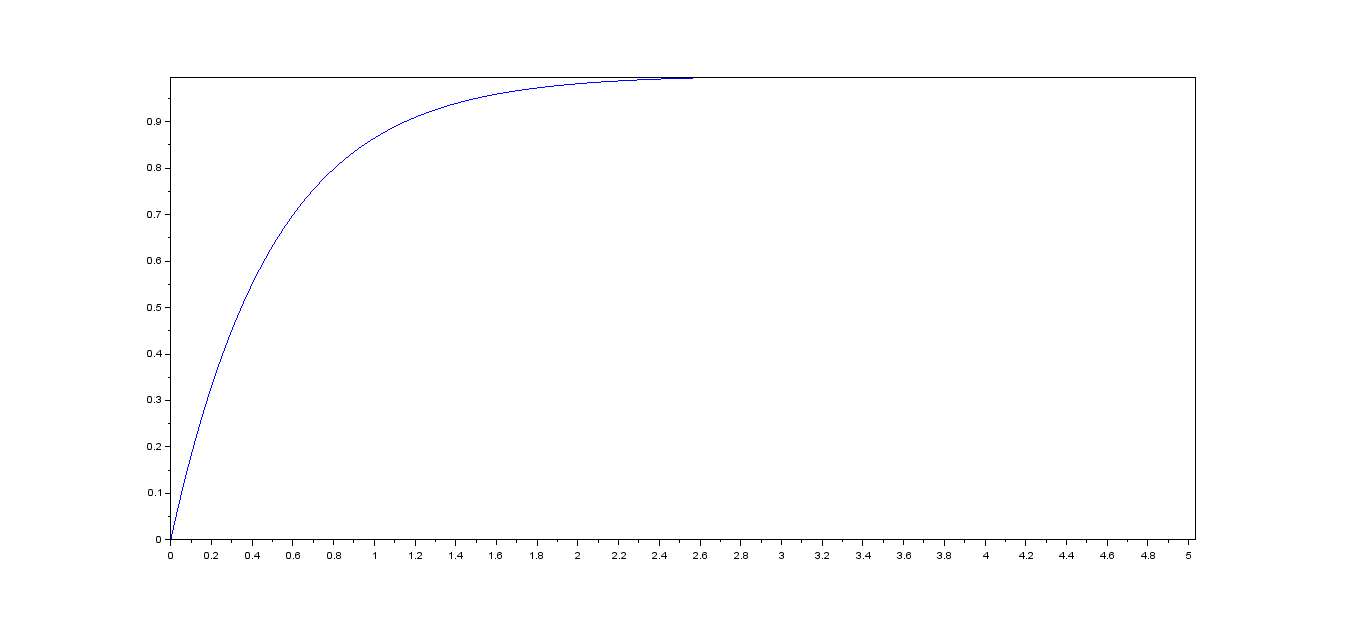
\includegraphics[scale=0.4]{CapitulosPrincipais/RespTransSistContinuos/Imagens/exemplo1.png}
\end{figure}
    
\end{document}